\documentclass[twocolumn]{aastex631}

% Packages
\usepackage{microtype}  % ALWAYS!
\usepackage{amsmath}
\usepackage{amsfonts}
\usepackage{amssymb}
\usepackage{multirow}
\usepackage{tikz}
\usepackage{xcolor}

\definecolor{pink}{RGB}{232,132,161}
\definecolor{yellow}{RGB}{255,213,0}

\newcommand{\kc}[1]{\textcolor{yellow}{\textbf{kc: #1}} }
\newcommand\shadetext[2][]{%
  \setbox0=\hbox{{\special{pdf:literal 7 Tr }#2}}%
  \tikz[baseline=0]\path [#1] \pgfextra{\rlap{\copy0}} (0,-\dp0) rectangle (\wd0,\ht0);% 
  }
\newcommand{\gb}[1]{\shadetext[left color=blue, right color=red, middle color=lime, shading angle=45]{\textbf{g: #1}} }
% \newcommand{\ecite}[1]{\textcolor{pink}{\textbf{: #1}} }
% \newcommand{\e}[1]{\textcolor{yellow}{\textbf{: #1}} }

\newcommand{\remove}[1]{\textcolor{red}{#1}}
\newcommand{\add}[1]{\textcolor{green}{#1}}

\newcommand{\mlg}{\ensuremath{M_{\rm LG}}}
\newcommand{\mmto}{\ensuremath{M_{\rm M31}}}
\newcommand{\mmw}{\ensuremath{M_{\rm MW}}}
\newcommand{\vtan}{\ensuremath{v_\textrm{tan}}}
\newcommand{\vrad}{\ensuremath{v_\textrm{rad}}}
\newcommand{\ms}[1]{\ensuremath{M_{*{#1}}}}
\newcommand{\mud}{\ensuremath{\mu_\delta}}
\newcommand{\mua}{\ensuremath{\mu_\alpha^*}}
\newcommand{\bov}{\ensuremath{\boldsymbol{v}}}
\newcommand{\boldx}{\ensuremath{\boldsymbol{x}}}
\newcommand{\vtrav}{\ensuremath{\bov_{\rm travel}}}
\newcommand{\xtrav}{\ensuremath{\boldx_{\rm travel}}}
\newcommand{\pos}[2]{\ensuremath{\boldx_{\rm #1 \to #2}}}
\newcommand{\vel}[2]{\ensuremath{\bov_{\rm #1 \to #2}}}
\newcommand{\mwbary}{\ensuremath{\textrm{MW}_\textrm{bary}}}
\newcommand{\mwouter}{\ensuremath{\textrm{MW}_\textrm{halo}}}
\newcommand{\mwdisk}{\ensuremath{\textrm{MW}_\textrm{disk}}}
\newcommand{\reflabel}[1]{\ensuremath{^{\mbox{\scriptsize{#1}}}}}

% Style tweaks
% \renewcommand{\twocolumngrid}{\onecolumngrid}
% \setlength{\parindent}{1.1\baselineskip}
% \sloppy\sloppypar\raggedbottom\frenchspacing

%%%%%%%%%%%%%%%%%%%%%%%%%%%%%%%%%%%%%%%%%%%%%%%%%%%%%%%%%%%%%%%%%%%%%%%%%%%%%%%%
\shorttitle{Frequency of galaxy pairs}
\shortauthors{Chamberlain et al.}

%%%%%%%%%%%%%%%%%%%%%%%%%%%%%%%%%%%%%%%%%%%%%%%%%%%%%%%%%%%%%%%%%%%%%%%%%%%%%%%%
\graphicspath{{./}{../plots/paper1/}}
% Missions
\newcommand{\project}[1]{\textsl{#1}}

% Packages / projects / programming
\newcommand{\package}[1]{\textsl{#1}}
\newcommand{\acronym}[1]{{\small{#1}}}
\newcommand{\github}{\package{GitHub}}
\newcommand{\python}{\package{Python}}
\newcommand{\astropy}{\package{Astropy}}

% Stats / probability
\newcommand{\given}{\,|\,}
\newcommand{\norm}{\mathcal{N}}
\newcommand{\pdf}{\textsl{pdf}}

% Maths
\newcommand{\dd}{\mathrm{d}}
\newcommand{\transpose}[1]{{#1}^{\mathsf{T}}}
\newcommand{\inverse}[1]{{#1}^{-1}}
\newcommand{\argmin}{\operatornamewithlimits{argmin}}
\newcommand{\mean}[1]{\left< #1 \right>}

% Non-scalar variables
\renewcommand{\vec}[1]{\ensuremath{\bs{#1}}}
\newcommand{\mat}[1]{\ensuremath{\mathbf{#1}}}

% Unit shortcuts
\newcommand{\Msun}{\ensuremath{\mathrm{M}_\odot}}
\newcommand{\Mjup}{\ensuremath{\mathrm{M}_{\mathrm{J}}}}
\newcommand{\kms}{\ensuremath{\mathrm{km}~\mathrm{s}^{-1}}}
\newcommand{\pc}{\ensuremath{\mathrm{pc}}}
\newcommand{\kpc}{\ensuremath{\mathrm{kpc}}}
\newcommand{\Mpc}{\ensuremath{\mathrm{Mpc}}}
\newcommand{\kmskpc}{\ensuremath{\mathrm{km}~\mathrm{s}^{-1}~\mathrm{kpc}^{-1}}}
\newcommand{\dayd}{\ensuremath{\mathrm{d}}}
\newcommand{\yr}{\ensuremath{\mathrm{yr}}}
\newcommand{\Myr}{\ensuremath{\mathrm{Myr}}}
\newcommand{\Gyr}{\ensuremath{\mathrm{Gyr}}}
\newcommand{\Kel}{\ensuremath{\mathrm{K}}}
\newcommand{\masyr}{\ensuremath{\mathrm{mas}~\mathrm{yr}^{-1}}}
\newcommand{\muasyr}{\ensuremath{\mu\mathrm{as}~\mathrm{yr}^{-1}}}

% Misc.
\newcommand{\bs}[1]{\boldsymbol{#1}}

% Astronomy
\newcommand{\DM}{{\rm DM}}
\newcommand{\feh}{\ensuremath{{[{\rm Fe}/{\rm H}]}}}
\newcommand{\df}{\acronym{DF}}

% TO DO
\newcommand{\todo}[1]{{\color{red} TODO: #1}}
\newcommand{\apw}[1]{{\color{blue} APW says: #1}}

% Projects
\newcommand{\gaia}{\textsl{Gaia}}
\newcommand{\gaiadr}{\textsl{Gaia}~\acronym{EDR3}}
\newcommand{\hst}{\textsl{HST}}
\newcommand{\ill}{\textsl{Illustris}}
\newcommand{\tng}{\textsl{IllustrisTNG}} 



% Affiliations
\newcommand{\affuofa}{University of Arizona, 933 N. Cherry Ave,
    Tucson, AZ 85721, USA}

%% This is the end of the preamble.  Indicate the beginning of the
%% manuscript itself with \begin{document}.

\begin{document}

\title{
  Frequency of dwarf and massive galaxy pairs in the IllustrisTNG cosmological simulation
}

\author[0000-0001-8765-8670]{Katie~Chamberlain}
\affiliation{\affuofa}

\author[0000-0003-0715-2173]{Gurtina Besla}
\affiliation{\affuofa}


\begin{abstract}
  \todo{REMEMBER TO USE 100-1000 REALS IN PLOTS}
  \todo{Include ticks on top and right axis as well}
\end{abstract}

%%%%%%%%%%%%%%%%%%%%%%%%%%%%%%%%%%%
\section{Introduction} \label{sec:intro}


%%%%%%%%%%%%%%%%%%%%%%%%%%%%%%%%%%%
%%%%%%%%%%%%%%%%%%%%%%%%%%%%%%%%%%%
\section{Sample selection}\label{sec:methods}
Our sample data was obtained using a strict set of selection criteria, as outlined in this section.
In Sec.~\ref{sec:methods-sims}, we provide motivation for and details of the simulations utilized in this study.
Sec.~\ref{sec:methods-am} explains the abudance matching prescription used to associate stellar masses with the dark matter subhalos.
Sec.~\ref{sec:methods-crit} provides a detailed outline of our selection criteria and process for picking pairs.
Finally, Sec.~\ref{sec:methods-counts} gives an overview of the properties of our sample.

%%%%%%%%%%%
%%%%%%%%%%%
\subsection{Simulation details}\label{sec:methods-sims}
% what is it that we are trying to study? why use illustris?
To understand the occurance rate and separations of typical galaxy pairs in a cosmological context, we require a simulation that provides a large statistical sample of pairs in both the dwarf and massive galaxy regime. 
Thus, we are limited in our simulation choice to large-volume cosmological simulations. 
However, we also require high resolution simulations such that the dwarf subhalos are resolved well enough to ensure robust statistics at the low mass end, and so we are not limited by our inability to resolve objects down to halo masses of $M_{\rm halo}\approx1\times 10^9\, \Msun$.

% Baryonic processes
Baryonic process are known to affect the dark matter halo structure of low mass ($M_*<1\times10^9\Msun$) subhalos in simulations~\citep[see e.g.][and references therein]{Sales:2022}.
Additionally, the shallow potential well of dwarf galaxies compared to their massive counterparts may lend themselves more easily to disruption from baryonic processes such as supernova feedback, which could change the occurance rate of low mass subhalos in hydrodynamic simulations \kc{check and see if they looked at this in the TNG100 galaxy paper}.
To study the effect of baryonic processes on the rate and separation of pairs, we require cosmological simulations which have both dark matter only runs and to full hydrodynamics.

% details of Illustris and Illustris TNG
The \textit{Illustris Project} ~\citep{vogelsberger14A,nelson15} and \textit{IllustrisTNG Project}~\citep{TNG1, TNG2, TNG3, TNG4, TNG5} are a set of N-body and hydrodynamic cosmological simulations which are perfectly suited for such a study. 
We use the dark matter only and full hydrodynamic runs of both the \ill-1 and \tng100-1 simulations to explore the connection between pairs and baryonic processes. 
Each of these simulations follows the dynamical evolution of $1820^3$ dark matter particles from $z=127$ to $z=0$ through a periodic volume of roughly $100^3$ Mpc$^3$. 
The \ill{} simulations follow a cosmology consistent with \textit{WMAP-9}~\citep{hinshaw13}, while the \tng{} simulations are consistent with \textit{Planck2015}~\citep{Planck2015}.
Specifically, we use the \textit{Illustris-1-Dark}, \textit{Illustris-1}, \textit{TNG100-1-Dark}, and \textit{TNG100-1} simulations (hereafter \illd, \illh, \tngd, and \tngh{} respectively, see Table~\ref{table:sim} for details).

% deets on the hydrodynamics of 
\kc{hydrodynamics details on the difference between the two hydro simulations. also include differences between the two dark simulations, if there are any besides the cosmology. }

% subfind, sublink, and groups and subhalos
We utilize the group catalogs produced by the \texttt{SUBFIND} algorithm ~\citep{springel01,dolag09}. 
These catalogs consist of halos (or "groups"), defined using the Friends-of-Friends (FoF) algorithm~\citep{davis85} to link nearby particles, and their associated subhalos, which are over-dense and gravitationally bound dark matter structures.
We also use the merger trees provided by the \texttt{SUBLINK} algorithm \citep{gomez15}, which tracks subhalos between snapshots using their particle data, in order to trace the mass growth and merger histories of our subhalos.


\begin{table*}[htb]
\begin{tabular}{l|llll}
 & \illd & \illh & \tngd & \tngh\\\hline\hline
 L$_{\rm Box}$ [Mpc] & 106.5 & 106.5 & 110.7 & 110.7 \\
m$_{\rm DM}$ [M$_\odot$] & 7.5$\times10^6$ & 6.3$\times10^6$ & 8.9$\times10^6$ & $7.5\times10^6$\\
m$_{\rm gas}$ & -- & $1.3\times 10^{6}$ & -- & $1.4\times 10^{6}$ \\\hline
\end{tabular}
\caption{\label{table:sim}Parameters of the Illustris simulations used in this analysis.}
\end{table*}



%%%%%%%%%%%
%%%%%%%%%%%
\subsection{Abundance matching prescription}\label{sec:methods-am}
% Why do we need stellar masses?
One of the goals of this study is to determine the impact of baryonic physics on the occurance rate and typical separations of galaxy \kc{subhalo?} pairs in cosmological simulations. 
However, selecting halo pairs by stellar mass ratio using the stellar masses provided by the simulations is not possible in the dark matter only runs. 
Thus, in order ensure the dark matter only and full hydrodynamic samples are self-consistent, we need to associate each of the selected subhalos with a realistic stellar mass.

% What is abundance matching
Abundance matching is one such method of associating a dark matter halo with a stellar mass, assuming a galaxy would form in a halo of that mass. 

However, there is large scatter in the stellar-mass-halo-mass (SMHM) relationship, especially in the dwarf halo regime. 



% How do we utilize it? 
In particular, we use the abundance matching relationship presented in~\citet{moster13}, which provides an analytic recipe to paint stellar masses onto dark matter halos. 
The~\citet{moster13} relationship is a redshift-evolving function of the halo mass, and includes terms to account for the systematic scatter in the SMHM relationship, with larger scatter at lower halo masses.
\kc{why moster instead of another AM relationship? most closely represent data at lower mass? }

To assign stellar masses to each of the dark matter halos, we assume that the stellar mass of both the primary and secondary halo can change as a function of redshift after the secondary has entered the primary's halo and do not immediately cease star formation.
This assumption is consistent with findings from~\cite{Akins2021}, which found that massive dwarf satellites ($M_*\approx 10^8-10^9\, \Msun$) entering MW-mass host halos are rarely quenched, and with~\cite{geha13} which finds that isolated dwarfs ($>1\Mpc$ from a MW-type galaxy) are often star forming and rarely quenched.
Additionally,~\citet{Munshi2021} found that the stellar mass of subhalos at $z=0$ in the XX simulations are more closely correlated with the peak halo mass than the $z=0$ halo mass for halos with peak halo mass $10^8<M_{\rm peak}<10^{11} \Msun$. 

Thus, we treat each of the subhalos as centrals according to the~\citet{moster13} prescription, using the current snapshot redshift and the peak halo mass of the subhalo to calculate the stellar mass. 
This additionally allows us remain robust to scenarios in which a secondary may have formed most of its stars, and then lost a significant portion of its dark matter content through tidal interactions with a primary, but will retain the bulk of its stellar content.

We create 1000 stellar mass realizations from the SMHM relationship, thus accounting for the systematic uncerntainy in subhalo stellar masses. Each realization is treated as an independent sample, such that computed properties (pair frequency, separations, etc) are given as the median each realization. We report the mean of all realizations and error bars indicate the 1$\sigma$ dispersion across the realizations.
%%%%%%%%%%%
%%%%%%%%%%%
\subsection{Selection criteria}\label{sec:methods-crit}
In this section, we outline the selection criteria used to select dwarf and massive subhalo pairs. 
The same selection criteria is utilized for all four simulations (\illd, \illh, \tngd, and \tngh)
In short, blah. 
Detailed steps are as follows. 

\subsubsection{Isolation}
As we are interested in the frequency and separations of galaxy pairs that are undisturbed by nearby massive perturbers, we select subhalo pairs as the most massive subhalos of their group halos. 
We have confirmed that nearly 100\% of the the most massive subhalos in each group are outside of the Hill radius of any nearby subhalo with greater mass, and are thus a rough isolation criteria is inherent in our selection.

\textbf{Definitions:} each of these defines the subhalo at a single snapshot and for a single realization.
\begin{itemize}
  \item Primary - Most massive subhalo in a group by stellar mass
  \item Secondary - 
  \item Major pair - A pair of subhalos consisting of a primary and secondary with stellar mass ratio $1/4 < \rm M_{*,sec}/M_{*, prim} < 1$
  \item Minor pair - A pair of subhalos consisting of a primary and secondary with stellar mass ratio $1/10 < \rm M_{*,sec}/M_{*, prim} < 1/4$
\end{itemize}
Note that the subhalo that is assigned as primary or secondary may change between stellar mass realizations. Also note\kc{that this method may yield pairs where the secondary has a higher subhalo mass than the primary. This one happens ~XX\% of the time.}

\begin{enumerate}
  \item Select groups in some group range that encompasses MCs and MW-M31
  \item For every subhalo in every group with halo mass >1e9Msun, use merger trees to get the maximum masses.
  \item Generate 1000 stellar mass realization using abundance matching so we can account for the spread in the relationship
  \item Generate catalog at each redshift containing: 
  \begin{itemize}
    \item For each realization, and in each group with a single subhalo, add the subhalo and it's properties to a catalog of single halos.
    \item For each realization, and in each group with 2+ halos, find most massive halo by stellar mass, and the second most massive halo by stellar mass, then add to pair catalog. 
    \item If a group has 3+ halos, check the stellar mass of the third most massive object, and see if it is a major/minor companion of the secondary. If not, teritary flag = 0. Otherwise =1.
  \end{itemize}
  \item Select dwarf primaries: for full catalog, most massive halo (in "pairs") or single halos with stellar mass $1\times10^{8} < \msam < 5\times10^{9} \Msun$. 
  \item Select dwarf pairs: for full pair catalog, any pair with stellar mass ratio between 1-1/4 (major pairs) or between 1/4-1/10 (minor pairs). All pairs is the union of these two sets. Any pair or single halo that is outside of these two sets is an "unpaired" halo. Note that unpaired can still have very minor companions. 
\end{enumerate}

The lower mass threshold for subhalos that constitute our dwarf pairs have a halo mass greater than $1\times10^9\Msun$, such that each of our halos are resolved into at least 100 particles in each simulation.  
\kc{why 100?} 

\subsubsection{Primary subhalos}\label{sec:methods-crit-prims}

\subsubsection{Primary subhalos}\label{sec:methods-crit-pairs}

\subsubsection{Stellar masses from the hydro sims}


\subsection{Counts and distributions}\label{sec:methods-counts}

\begin{itemize}
  \item Introduce simulations
  \item outline selection steps
  \item dwarf pairs
  \item massive pairs
  \item include table with parameters used for pairs
  \item plots
    \begin{itemize}
      \item distribution plots
      \item counts plots
    \end{itemize}
\end{itemize}


% selection criterion
\begin{table*}[htb]
  \centering
    \begin{tabular}{lcc}
     & Dwarf Pairs & Massive Pairs \\\hline\hline
    % Group Mass & $8\times10^{10} < \rm M_g < 5\times10^{11} M_\odot$ & $1\times10^{12} < \rm M_g < 4\times10^{12} M_\odot$  \\
    % Subhalo Max Mass &  &  \\
    % Subhalo Current Mass & $>1\times10^{10} \Msun$ & $> 5\times10^{11} \Msun$ \\
    Primary &$1\times10^{8} < \msam < 5\times10^{9} \Msun$ & $5\times10^{9} < \msam < 1\times10^{11} \Msun$\\\hline
    \end{tabular}
    \caption{\label{table:mass}Selection criteria for dwarf and massive pairs.}
    \end{table*}

% equivalent snapshot table
\begin{table*}[]
  \centering
  \begin{tabular}{l|cc|cccc} % increase this to 7 columns
    \hline \hline
   & \multicolumn{2}{c|}{Snapshot number} & \multicolumn{4}{c}{Number of primaries}\\
   & \ill & \tng  & \illd & \illh & \tngd & \tngh \\ 
  \hline
  z = 0   &   135  &   99   & $11431.5_{-24.42}^{68.38}$ & $12650.0_{-25.84}^{46.84}$ & $13255.0_{-32.60}^{56.72}$ & $12035.0_{-69.24}^{20.36}$\\
  z = 1   &   85   &   50   &  $14769.0_{-30.24}^{47.28}$ & $16568.0_{-32.20}^{69.60}$ & $17445.5_{-40.86}^{51.90}$ & $15946.5_{-59.38}^{39.22}$ \\
  z = 2   &   68   &   33   &  $12602.5_{-31.98}^{45.94}$ & $14174.0_{-12.48}^{62.32}$ & $15413.5_{-34.62}^{28.86}$ & $14334.0_{-29.44}^{45.24}$ \\
  z = 3   &   60   &   25   &     $8533.5_{-54.50}^{39.46}$ & $9390.0_{-63.40}^{41.32}$ & $10901.0_{-44.64}^{46.56}$ & $10106.5_{-47.90}^{39.74}$  \\
  % z = 3.7   &   54   &   21   \\
  \hline \hline
  \end{tabular}
  \caption{\label{tab:equiv-snapshot} The snapshot number of the original \ill\ and the \tng\ simulations at redshifts $z=0-3$, as well as the median number dwarf (massive) primaries that were selected with $1\times 10^{8} < \msam < 5\times 10^{9} \rm M_\odot$ ($5\times 10^{9} < \msam < 1\times 10^{11} \rm M_\odot$) in XX abundance matching realizations. \kc{fill in with numbers after doing more realizations} \kc{include takeaway}}
  \end{table*}

  \begin{figure*}[htb]
    \centering
    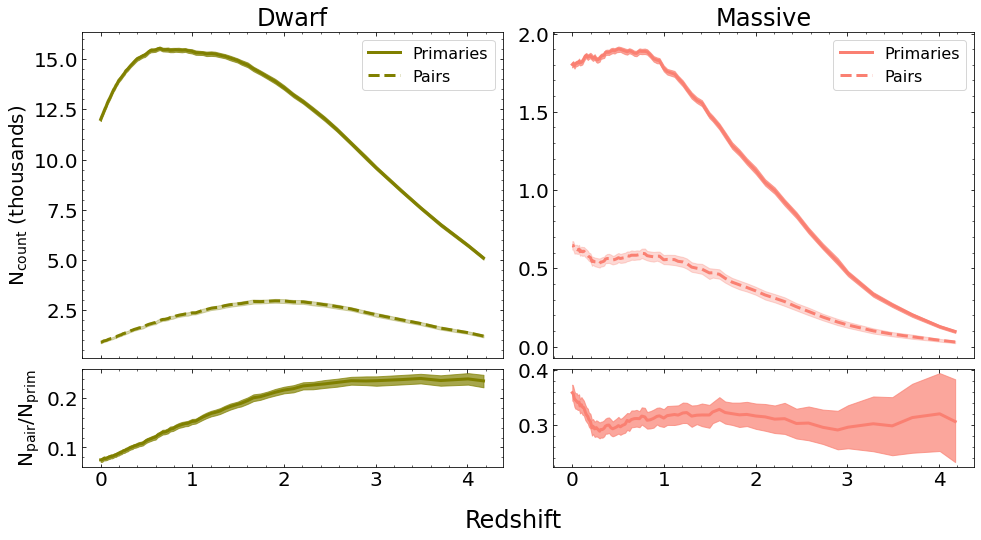
\includegraphics[width=\textwidth]{counts_1000.png}
    \caption{(Top) Median number of dwarf (left) and massive (right) primaries and pairs per abundance matching realization as a function of redshift.
    Shaded regions show the $1^{\rm st}$ and 99$^{\rm th}$ percentile spread of the medians of all realizations. 
    There are approximately 8 times as many dwarf primaries as massive primaries. 
    % dwarf galaxies
    The dwarf primary count (green solid line in top left panel) is at a minimum at $z=4$, rises to a maximum of $\sim15000$ halos per realization by $z=1$, then decreases by $\sim16\%$ to 12000 halos at $z=0$. The dwarf pair count (green dashed line), on the other hand, peaks at $z\sim2$ with 3000 pairs, and decreases to a minimum of about 1000 pairs at $z=0$.
    % Massive galaxies (right)
    The massive primary count (pink solid line in top right panel) behaves similarly to the dwarf primary count, with a minimum count at $z=4$ which rises to a maximum of $\sim2000$ halos per realization at $z\sim1$, then decreases slightly by $\sim5\%$ to $\sim$1800 halos by $z=0$. 
    Unlike dwarf pairs whose pair count peaks at $z=2$, pair count for massive galaxies (pink dashed line) follows similar behavior to the total massive primary count, with a minimum at $z=4$, and increasing to $z=\sim 1$ before leveling off. At very low redshift, the pair count and primary count have opposite behavior, with the pair count \textit{increasing} at very low redshifts of $z=0-0.25$ and \textit{peaking} at $z=0$.
    (Bottom) Fraction of pairs per primary as a function of redshift (i.e., the ratio between dotted line and solid line in each column). Dwarf and massive pair fractions are roughly flat for $z=2.5-4$, but display opposite behavior for $z=0-2.5$. The dwarf pair fraction decreases steadily from $\sim0.24$ to $\sim0.08$, a decrease of roughly $65\%$, while the massive pair fraction is roughly flat between $z=1-2.5$ with an average of $0.31$, before spiking sharply from $\sim 0.29$ to $\sim 0.36$ between $z=0-0.25$, an increase of $25\%$.}
    \label{fig:counts}
  \end{figure*}

  \begin{figure*}[htb]
    \centering
    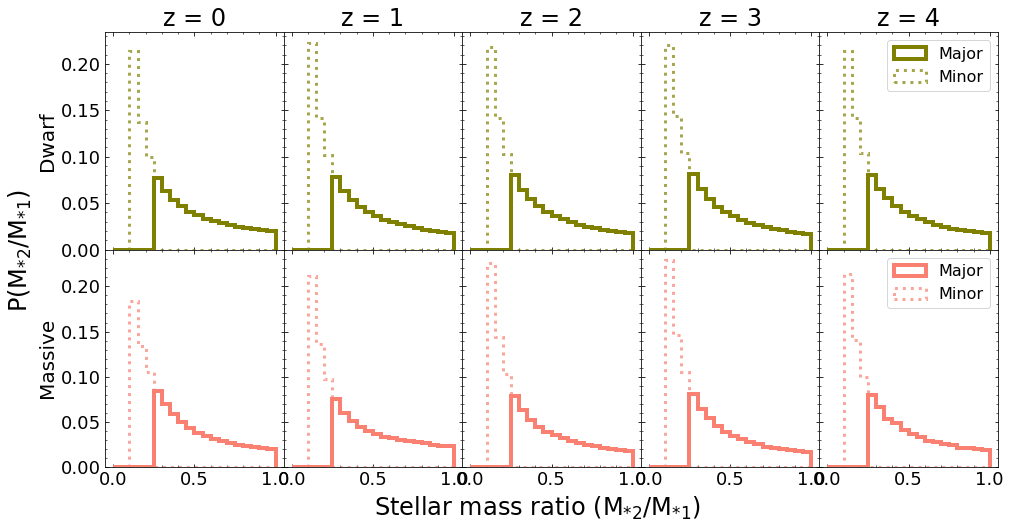
\includegraphics[width=\textwidth]{stellarmass_distribution_1000.png}
    \caption{Stellar mass ratio distribution of all dwarf (top) and massive (bottom) pairs. Major pairs (solid lines) are defined as pairs with mass ratio $\ms{2}/\ms{1} > 1/4$, while minor pairs (dotted lines) are defined as pairs with stellar mass ratio $1/10<\ms{2}/\ms{1}<1/4$. Overall, the stellar mass ratio distribution of major and minor pairs of dwarf and massive galaxies show little evolution from $z=4$ (right) to $z=0$ (left). 
    Major pairs make up $51-55\%$ of the full sample of pairs at every redshift for both dwarf and massive pairs.}
    \label{fig:massratio}
  \end{figure*}



%%%%%%%%%%%%%%%%%%%
%% dwarf figures %%
%%%%%%%%%%%%%%%%%%%
\kc{why did we stop at z=4? we didn't, explanation about low \# statistics }

%%%%%%%%%%%%%%%%%%%%%%%%%%%%%%%%%%%

\section{Results}
We collect dwarf pairs and massive pairs at all snapshots from the TNG100-1 simulation and analyze the occurrence rate and kinematic behavior of the pairs across cosmic time. 
At each snapshot, we generate 1000 different realizations of the pair catalog, where each realization represents one instance of the abundance matching technique to assign stellar masses to dark matter halos (see methods). 
In each of the following plots, the median and a percentile spread each value are calculated by finding the median from each of the 1000 AM realizations, and taking the median and spread of that set of median values.

In Sec.~\ref{sec:results-frac}, we show the redshift evolution of the fraction of primaries with a major or minor companion and compare the "pair fractions" of dwarf pairs to massive pairs.
In Sec.~\ref{sec:results-kinematics}, we look at the redshift evolution of the median separations and relative velocities between primary and secondary halos on a snapshot-by-snapshot basis.


\subsection{Pair fraction}\label{sec:results-frac}
Thus, the rate of dwarf pairs and massive pairs \textit{per primary} will evolve distinctly in the dwarf and massive pair case.

\label{sec:results}
\begin{figure*}[htb]
  \centering
  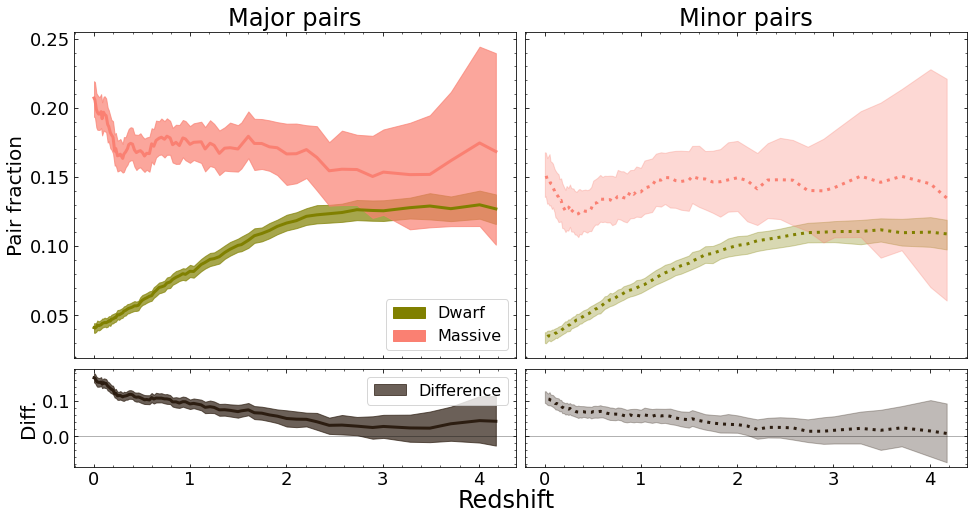
\includegraphics[width=\textwidth]{pairratio_1000.png}
  \caption{
    % Top plots ~
    (Top) Median fraction of dwarf or massive primaries with a major or minor companion by stellar mass. 
    Shaded regions show the $1$-$99$ percentile range of the median pair fractions of each realization. 
      % massive pairs
    The fraction of massive primaries (pink) with a major (left) or minor (right) companion remains approximately constant for $z>1$, with an average pair fraction of 0.16-0.17 and 0.14-0.15 respectively. Between $z=0.25$ and $z=0$, the massive major pair fraction increases sharply from 0.165 to 0.207, a 25\% increase, while the minor pair fraction increases from 0.127 to 0.152, a 20\% increase.
      % dwarf pairs
    Dwarf pairs (green), on the other hand, have pair fractions that are approximately constant from $z=3-4$, but the fraction of major(minor) pairs declines monotonically from 0.126(0.111) at x=3 to just 0.041(0.034) at x=0, a 67(70)\% decrease. 
    % Bottom plots ~
  (Bottom) The median subtracted difference between the massive pair fraction and the dwarf pair fraction, with the shaded $1$-$99$ percentile range of the difference of each realization. The difference between the massive pair fraction and dwarf pair fraction increases with decreasing redshift, peaking at $z=0$ with a difference of 0.166 for major pairs and 0.111 for minor pairs. This shows that the redshift evolution of the pair fractions of massive pairs and dwarf pairs proceed differently, particularly in the low redshift regime.}
  \label{fig:pairratio}
\end{figure*}

\subsection{Kinematic evolution}\label{sec:results-kinematics}
The primary and secondary halos of each pair at each individual snapshot/redshift is separated by some physical separation and has a relative velocity of 

We separate the population of dwarf and massive pairs into "major" and "minor" pairs (as defined in Sec.~\ref{sec:methods-crit-pairs}) to show how the stellar mass ratio between the primary and secondary may affect the kinematics. 

At each individual snapshot, we find the instantaneous median separation and relative velocity of every pair that was selected in that snapshot. 

\subsubsection{Separations}
% separation vs. redshift plot
The median separations of dwarf pairs and massive pairs smoothly increases with lower redshift, regardless of pair type. 
Fig.~\ref{fig:sep} shows the median and 1-99\% range of separations for dwarf pairs and massive pairs, as well as the subtracted difference between the median separation of major pairs and of minor pairs of both mass type. 
There is a small offset in the median separations of major and minor dwarf pairs (between $10-25\,\kpc$ from  $z=0-1$ and approximately $5\,\kpc$ from $z=1-4$), and a larger median separation offset for major and minor massive pairs (between $25-100\,\kpc$ from  $z=0-1$ and approximately $10-40\,\kpc$ from $z=1-4$). 
Thus, apart from the overall scale of the separations between primary and secondary, dwarf and massive pairs exhibit similar trends as a function of time. 

% separation distribution plot
Fig.~\ref{fig:sep-dist} shows the full distribution of separations for major and minor dwarf and massive pairs at $z=\{0,1,2,3,4\}$, and includes all 1000 AM realizations. 
For reference, the median at each corresponding redshift from Fig.~\ref{fig:sep} (that is, the median of the medians of each realization) are shown in light black vertical lines.
Each plot is normalized such that the area under an individual curve is 1.
    % the redshift evolution
All pair types (dwarf and massive, major and minor) have narrow distributions that pile up around 0 $\kpc$ at $z=4$, but the distributions become more and more broad as $z\to0$ (note that only pairs with separations $>10\kpc$ are included in this analysis, see Sec.~\ref{sec:methods-crit-pairs}).

The distribution profiles are similar when the scale of the x-axis for massive pair separations is twice that of the dwarf pairs. 
Pair separations at $z=0$ tend to primarily fall between $10-\sim400\,\kpc$ for dwarf pairs and   between $10-\sim1000\,\kpc$ for massive pairs. 
At $z=4$, these ranges decrease to $10-150\,\kpc$ for dwarf pairs and $10-300\,\kpc$ for massive pairs. 
    % comparing major and minor
Major and minor pairs (both dwarf pairs and massive pairs) have roughly equivalent distributions, though the distribution of minor pairs with low separations is slightly higher than the major pairs. Thus, secondary halo of minor pairs tend to live slightly closer to their primaries than the  major secondaries.

\todo{here maybe include a table? what are some values?  z=0,1,2,3,4 and pair frac, sep, vel. ?}



\subsubsection{Relative Velocities}
% velocity vs. redshift plot
We also consider the snapshot-by-snapshot instantaneous relative velocity between each primary and secondary.
We find that the median relative velocity of all pairs (dwarf and massive, major and minor) decreases with decreasing redshift, reaching a minimum at $z=0$ as seen in Fig.~\ref{fig:vel}. 
Though the velocity scales are different, the bulk behavior of dwarf pairs and massive pairs is identical. 

The median velocity of a major dwarf pair decreases approximately linearly from $xx$ at $z=4$ to $xx$ at $z=0$. Likewise, the median velocity for major massive pairs decreases.
Fig.~\ref{fig:vel} also includes a panel showing the subtracted median difference at each snapshot of the minor pair from the major pair. Since minor pairs typically have slightly higher velocities than their major pair counterparts, this difference is usually $<\sim0$. 

% velocity distribution plot
Fig.~\ref{fig:vel-dist}



%%% plots for kinematics
\begin{figure*}[htb]
  \centering
  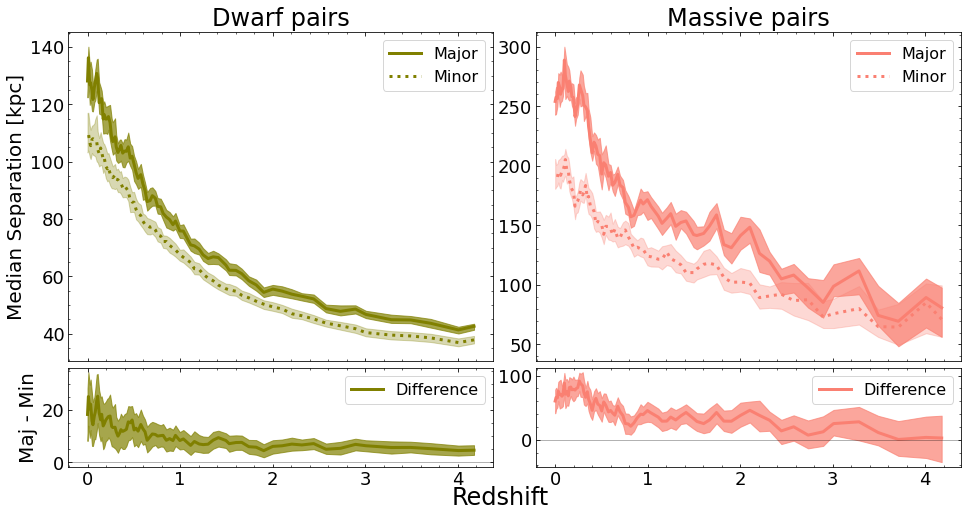
\includegraphics[width=\textwidth]{separation_1000.png}
  \caption{(Top) Median physical separation (in kpc) of dwarf pairs (left, green) and massive pairs (right, pink) as a function of redshift. 
  Shaded areas show the 1-99 percentile range of the median from 1000 abundance matching realizations. 
  Major pairs (high stellar mass ratio) are shown in solid lines, while minor pairs are depicted with dashed lines.
  In general, as the redshift decreases from $z=4$ to $z=0$, the average physical separation of a pair increases for both dwarf and massive pairs. 
  % Dwarf pairs
  The redshift evolution of the dwarf pairs closely resembles a power law distribution across the whole redshift range from $z=0-4$.
  At $z=4$, the typical separation between major (minor) dwarf pairs is $42(38)\,\kpc$, and peaks at $z=0$ with a median separation of $128(109)\,\kpc$.
  % Massive Pairs
  The separation between massive pairs, on the other hand, increases approximately linearly from $z=4$, where the median separations of major (minor) pairs is $81(71)\,\kpc$, to $z=1$, where median separations are $171(124)\,\kpc$. The median separation rises more steeply from z=1 to z=0, peaking around $z=\sim0$ at $288\,\kpc$ and $205\,\kpc$ for major and minor massive pairs respectively.
  % Difference plots
  (Bottom) The median subtracted separation difference between major and minor pairs, and 1-99\% shaded region.
  Minor dwarf pairs tend to be $\sim10-20\kpc$ closer to their primary than major dwarf pairs, while minor massive pairs are between $10-50\kpc$ closer than major pairs. 
    }
  \label{fig:sep}
\end{figure*}

\begin{figure*}[htb]
  \centering
  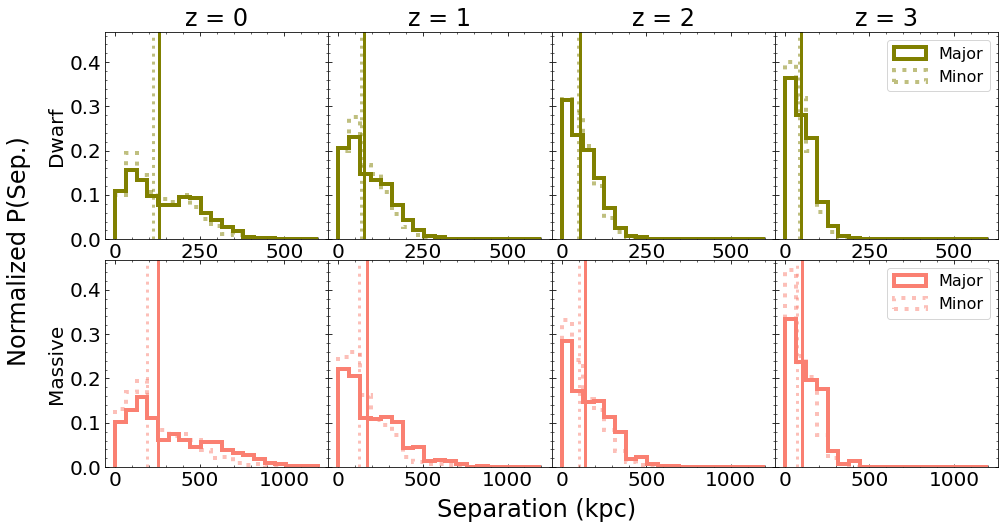
\includegraphics[width=\textwidth]{separation_distribution.png}
  \caption{Normalized physical separation distribution for dwarf (top) and massive (bottom) pairs from $z=0$ (left) to $z=4$ (right). Major pairs are shown as solid lines, while minor pairs are dotted. The median separation of each pair type from the previous plot is shown in solid (major) and dotted (minor) vertical black lines. 
  At higher redshift $z=3-4$, a large fraction of both dwarf and massive pairs have low separations ($<$ 125 \& 250 $\kpc$ respectively). However, at low redshift, the separation distribution tends to spread out more evenly across a large range of separations, thus increasing the median.
  % \kc{would it be instructive to make this plot, unnormalized, with z=0-3 on same plot to see if low sep pop numbers change drastically}
   \todo{change color of med lines, add z=4, replace with 1000 reals }
    }
  \label{fig:sep-dist}
\end{figure*}

\begin{figure*}[htb]
  \centering
  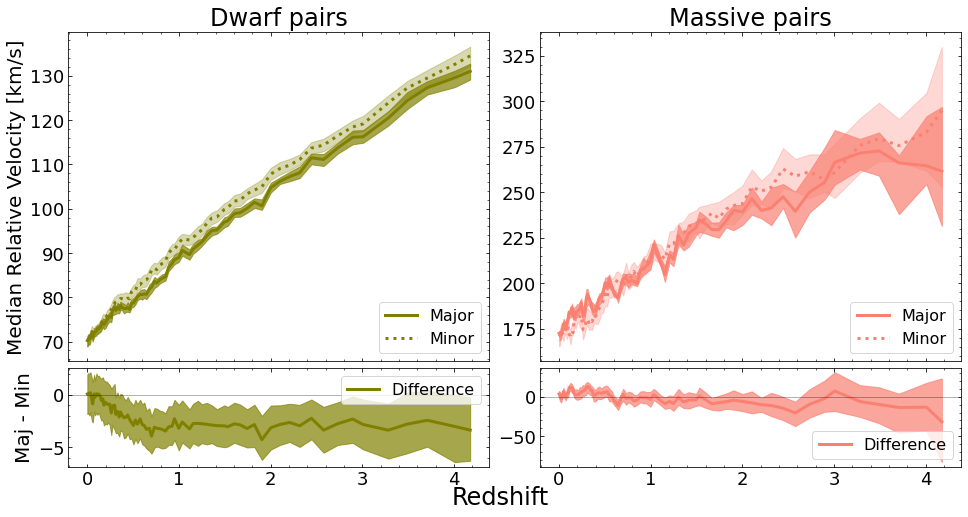
\includegraphics[width=\textwidth]{velocity_1000.png}
  \caption{
    (Top) Median relative velocity (in \kms) between the primary and secondary halos of: dwarf pairs (left, green), and massive pairs (right, pink) as a function of redshift. 
    Shaded areas show the 1-99 percentile range of the median from 1000 abundance matching realizations. Major pairs (high stellar mass ratio) are shown in solid lines, while minor pairs are depicted with dashed lines.
    The overall behavior of the redshift evolution is nearly identical for dwarf and massive pairs.
    As the redshift decreases from $z=4$ to $z=0$, the average relative velocity of a pair decreases as well for both dwarf and massive pairs.
    % brief describe
    The median relative velocity of a dwarf pair (major or minor) is $70\,\kms$ at $z=0$ and $133\,\kms$ at $z=4$, and of a massive pair is $170\,\kms$ at $z=0$ and $260\,\kms$ at $z=4$ ($295\,\kms$ for a minor pair). 
    % Difference plot
    (Bottom) The median subtracted relative velocity difference between major and minor pairs, and 1-99\% shaded region.
    The is little difference between major and minor dwarf pairs (bottom left), with minor pairs having a relative velocity of $0-5\,\kms$ higher than major pairs. 
    Major and minor massive pairs also have very little median velocity difference at low redshift (bottom right), with minor pairs having a relative velocity between $1-20\,\kms$ faster than major pairs.
    }
  \label{fig:vel}
\end{figure*}

\begin{figure*}[htb]
  \centering
  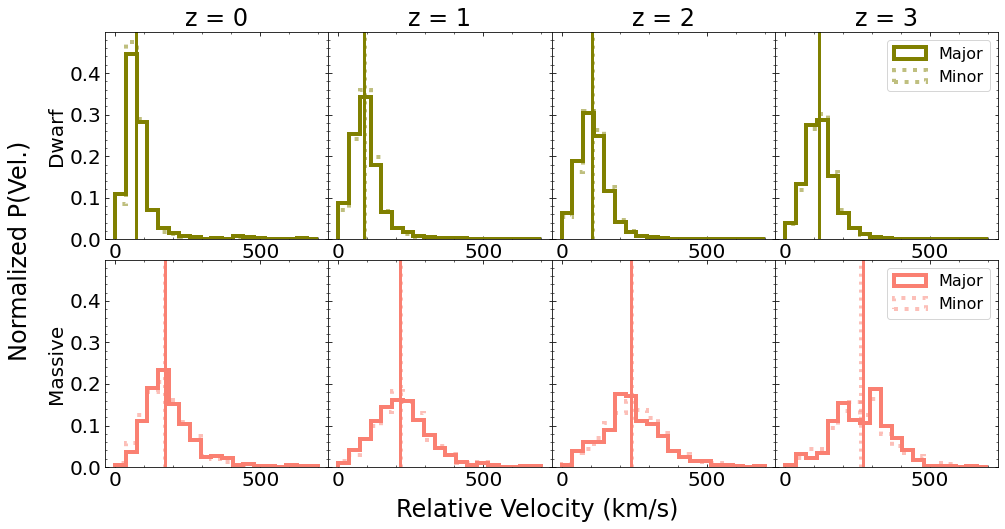
\includegraphics[width=\textwidth]{velocity_distribution.png}
  \caption{
  Normalized distribution of relative velocities between primary and secondary halos for dwarf (top) and massive (bottom) pairs from $z=0$ (left) to $z=4$ (right). Major pairs are shown as solid lines, while minor pairs are dotted. The median separation of each pair type from the previous plot is shown in solid (major) and dotted (minor) vertical black lines. 
  %
  The distribution of relative velocities for dwarf and massive pairs move to slightly lower velocities at lower redshifts. The distribution of velocities for major and minor pairs is roughly equivalent. 
  \todo{finish caption, change color of med lines, add z=4, replace with 1000 reals}
    }
  \label{fig:vel-dist}
\end{figure*}
%%%




%%%%%%%%%%%%%%%%%%%%%%%%%%%%%%%%%%%
\section{Discussion}
\label{sec:discussion}

Pair ratio fig. -- The vast difference between the dwarf and massive pair fractions suggests \todo{XX - that pairs at different mass scales evolve differently ? Thus, can't just assume a massive pair fraction for a lower mass regime} 

Mean separation fig. -- The increase in low redshift median separations suggests that low separation pairs undergo mergers that remove them from the sample at later snapshots, thus increasing the median separation over time.

Separation dist fig. -- The number of widely separated pairs at low redshift is much greater than at high redshift, so these pairs either form late, or move apart from each other. 

Scaled sep fig. -- \textbf{The difference between the scaled separations of dwarf and massive pairs highlights the mass dependence of the physical distribution of halo pairs, i.e., dwarf pairs are not simply a smaller scale version of massive pairs.}

Scaled vel fig. --   \textbf{Despite the difference between dwarf and massive pairs in physical distribution as indicated by the plot of scaled separations (Figure~\ref{fig:sep-scaled}), the scaled velocity distribution of pairs indicates that dwarf and massive galaxy pairs operate similarly in velocity space. There is little to no mass dependence on the scaled velocity of dwarf or massive pairs.}
Also note than many of the close pairs at high z may merge by $z=0$.

\begin{figure*}[htb]
  \centering
  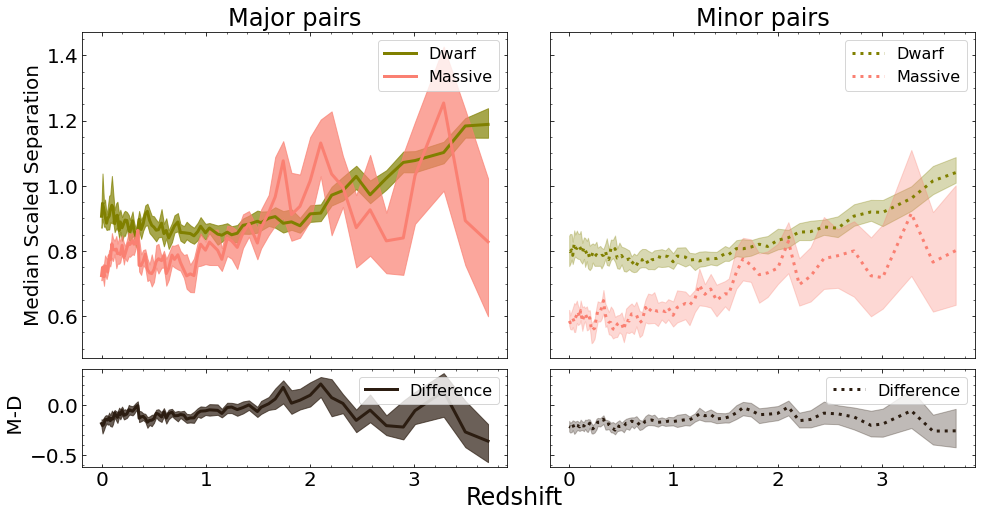
\includegraphics[width=\textwidth]{scaledsep.png}
  \caption{Median scaled separation (separation of a pair divided by the virial radius of its group) as a function of redshift. Dwarf pairs (major (solid) and minor (dashed)) tend to have smaller scaled separations at lower redshifts, leveling out between $z=0-1$. In particular, the secondaries of dwarf major pairs at $z>2$ tend to live more than one virial radius away from the primary. Massive major pairs at low redshift tend to have smaller scaled separations  at $z<\sim2$, but vary significantly at higher redshifts. 
  Minor pairs (right), both dwarf and massive, tend to have smaller separations, tending to live closer than one virial radius between the primary and secondary. Massive minor pairs tend to have smaller scaled separations compared to dwarf pairs at all redshifts.
  \todo{replace with 1000 reals fig, finish caption, add 0 horizon line}
    }
  \label{fig:sep-scaled}
\end{figure*}

\begin{figure*}[htb]
  \centering
  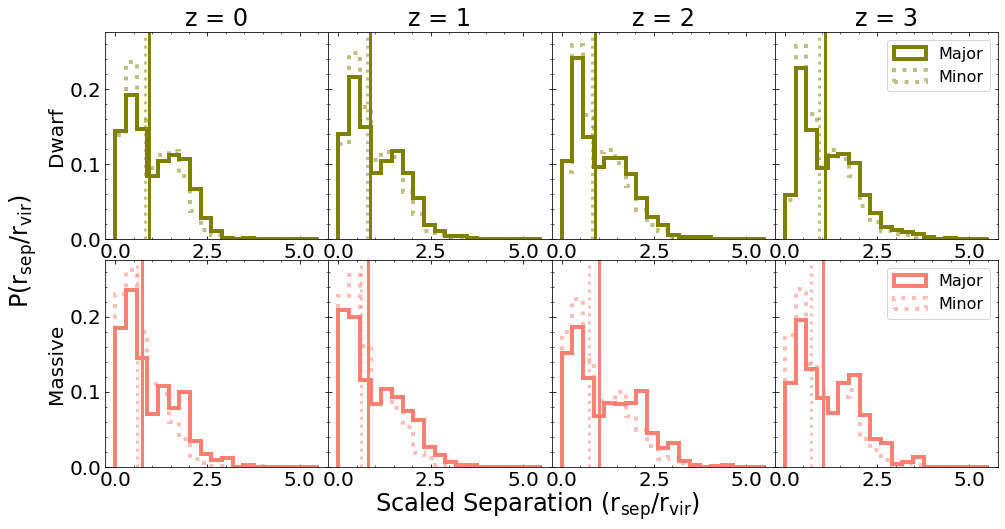
\includegraphics[width=\textwidth]{scaledsep_distribution.png}
  \caption{\todo{finish caption, 1000 reals, change median color, add z=4}}
  \label{fig:sep-scaled-dist}
\end{figure*} 


\begin{figure*}[htb]
  \centering
  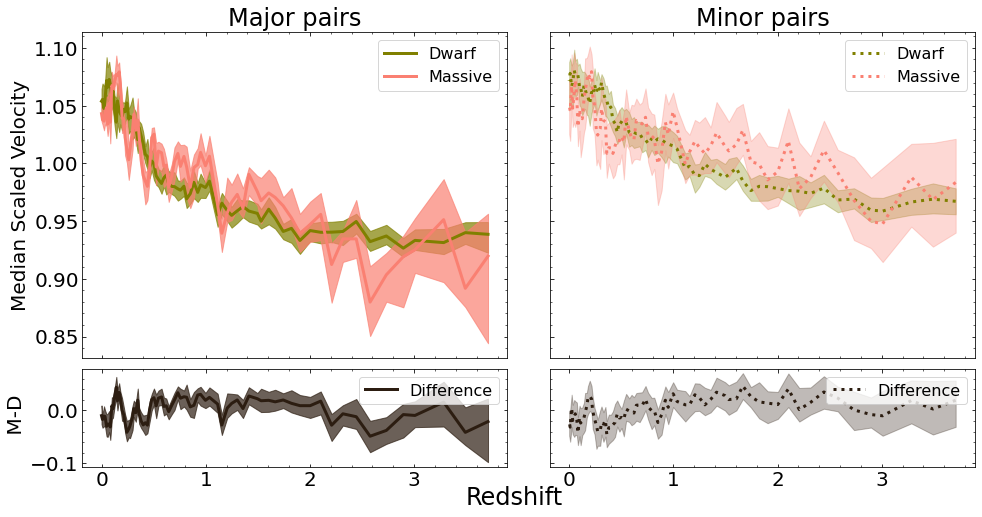
\includegraphics[width=\textwidth]{scaledvel.png}
  \caption{Median scaled velocity (relative velocity of a pair divided by the virial velocity), defined as the circular velocity at the virial radius of the group as a function of redshift. 
  Major pairs are on the left (solid lines), minor pairs are on the right in dashed lines.
  All sets of pairs show an increase in scaled velocity at lower redshifts.
  \todo{finish caption, replace with 1000 reals, add 0 horizon line}
  }
  \label{fig:vel-scaled}
\end{figure*} 

\begin{figure*}[htb]
  \centering
  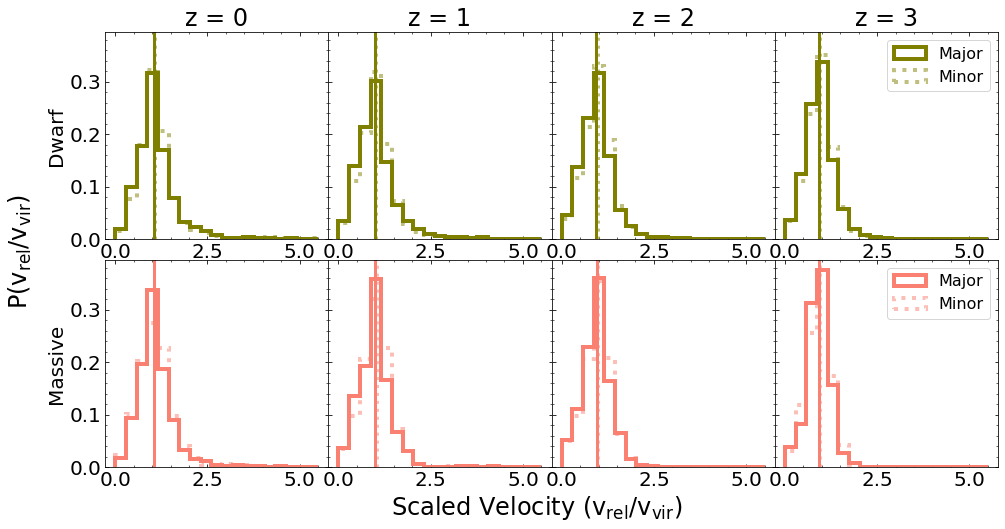
\includegraphics[width=\textwidth]{scaledvel_distribution.png}
  \caption{\todo{finish caption, 1000 reals, change median color, add z=4}}
  \label{fig:vel-scaled-dist}
\end{figure*} 


\kc{add discussion subsection titles}
\subsection{Dwarf and massive pair kinematic differences}
\subsection{Comparison to literature}
\subsection{Implications for observations}


%%%%%%%%%%%%%%%%%%%%%%%%%%%%%%%%%%%
\section{Summary and Conclusions}
\label{sec:summary}

%%%%%%%%%%%%%%%%%%%%%%%%
%%%%%%%%%%%%%%%%%%%%%%%%

\bibliography{refs}{}
\bibliographystyle{aasjournal}

\end{document}
